\documentclass[11pt]{article}
\usepackage[margin=1in]{geometry}
\usepackage{graphicx}
\usepackage{booktabs}
\usepackage{caption}
\usepackage{hyperref}
\usepackage{fancyhdr}
\pagestyle{fancy}
\lhead{W95--W104 Report}
\rhead{SSWD Calibration}

\title{Calibration Report: Pathogen Thermal Adaptation\\(W95--W104)}
\author{Anton Star --- SSWD-EvoEpi Project}
\date{March 5, 2026}

\begin{document}
\maketitle

\section{Executive Summary}
W95--W104 are the first calibration runs with \textbf{pathogen thermal adaptation} enabled --- a mechanism allowing each node's VBNC threshold ($T_\mathrm{vbnc}$) to evolve downward as cold-adapted pathogen strains are selected.

\textbf{Key finding:} Thermal adaptation is negligible at tested rates. Even at the highest adaptation rate (W98, $r=0.005$), $T_\mathrm{vbnc}$ shifted by only 0.14\textdegree C at AK-PWS (from 12.0 to 11.86). JDF and SS-S showed $<$0.02\textdegree C change. The mechanism does not operate on the 13-year simulation timescale.

\textbf{Best run: W99} (floor=500, $\alpha$=0.20, adapt=0.001) achieves RMSE=0.557 --- our best ever. However, this is driven by the floor/$\alpha$ combination, not adaptation. AK-PWS remains at 10.8\% (target 50\%).

\section{Methods}
All runs share: $K_{1/2}$=800K, CDT=1000, wfDP=300, wfRange=3000, dynamic $P_\mathrm{env}$, $\delta$=0.02, revert\_rate=0.0005.

\begin{table}[h]
\centering
\small
\begin{tabular}{lcccc}
\toprule
Run & Floor & $\alpha$ & Adapt Rate & $T_\mathrm{vbnc,min}$ \\
\midrule
W90 (ref) & 300 & 0.20 & --- & --- \\
W91 (ref) & 500 & 0.20 & --- & --- \\
\midrule
W95 & 300 & 0.20 & 0.0005 & 6 \\
W96 & 300 & 0.20 & 0.001 & 6 \\
W97 & 300 & 0.20 & 0.002 & 6 \\
W98 & 300 & 0.20 & 0.005 & 6 \\
W99 & 500 & 0.20 & 0.001 & 6 \\
W100 & 500 & 0.20 & 0.002 & 6 \\
W101 & 300 & 0.20 & 0.001 & 8 \\
W102 & 300 & 0.20 & 0.001 & 4 \\
W103 & 300 & 0.15 & 0.001 & 6 \\
W104 & 200 & 0.15 & 0.001 & 6 \\
\bottomrule
\end{tabular}
\end{table}

\section{Results}

\begin{table}[h]
\centering
\small
\begin{tabular}{lccccccccr}
\toprule
Run & AK-PWS & AK-FN & AK-FS & BC-N & SS-S & JDF & OR & CA-N & RMSE \\
 & (50) & (50) & (20) & (20) & (5) & (2) & (0.25) & (0.1) & \\
\midrule
W90 & 10.5 & 4.8 & 6.0 & 6.9 & 5.8 & 1.9 & 0.9 & 1.0 & 0.643 \\
W91 & 11.3 & 5.7 & 2.6 & 9.3 & 7.4 & 5.9 & 0.5 & 0.3 & 0.591 \\
\midrule
W95 & 10.6 & 4.6 & 4.2 & 8.4 & 9.3 & 19.7 & 1.0 & 1.6 & 0.790 \\
W96 & 11.3 & 5.3 & 6.4 & 8.5 & 4.0 & 9.2 & 1.4 & 0.6 & 0.649 \\
W97 & 9.9 & 7.0 & 12.0 & 7.7 & 5.4 & 2.0 & 3.0 & 0.8 & 0.654 \\
W98 & 12.1 & 6.0 & 3.6 & 8.6 & 4.8 & 15.4 & 1.4 & 0.8 & 0.709 \\
\textbf{W99} & \textbf{10.8} & \textbf{8.8} & \textbf{6.2} & \textbf{8.4} & \textbf{2.9} & \textbf{4.3} & \textbf{1.0} & \textbf{0.6} & \textbf{0.557} \\
W100 & 10.1 & 4.1 & 3.7 & 8.1 & 4.4 & 3.3 & 2.3 & 0.5 & 0.687 \\
W101 & 11.3 & 5.3 & 6.4 & 8.5 & 4.0 & 9.2 & 1.4 & 0.6 & 0.649 \\
W102 & 11.3 & 5.3 & 6.4 & 8.5 & 4.0 & 9.2 & 1.4 & 0.6 & 0.649 \\
W103 & 20.8 & 9.4 & 8.0 & 13.6 & 6.8 & 19.6 & 6.7 & 4.9 & 0.919 \\
W104 & 24.9 & 6.1 & 10.2 & 14.0 & 15.2 & 28.5 & 6.0 & 5.6 & 0.972 \\
\bottomrule
\end{tabular}
\caption{Recovery fractions (\%) by region. Targets in parentheses. W99 bolded as best RMSE.}
\end{table}

\subsection{Key Runs: Recovery Time Series}
\begin{figure}[h]
\centering
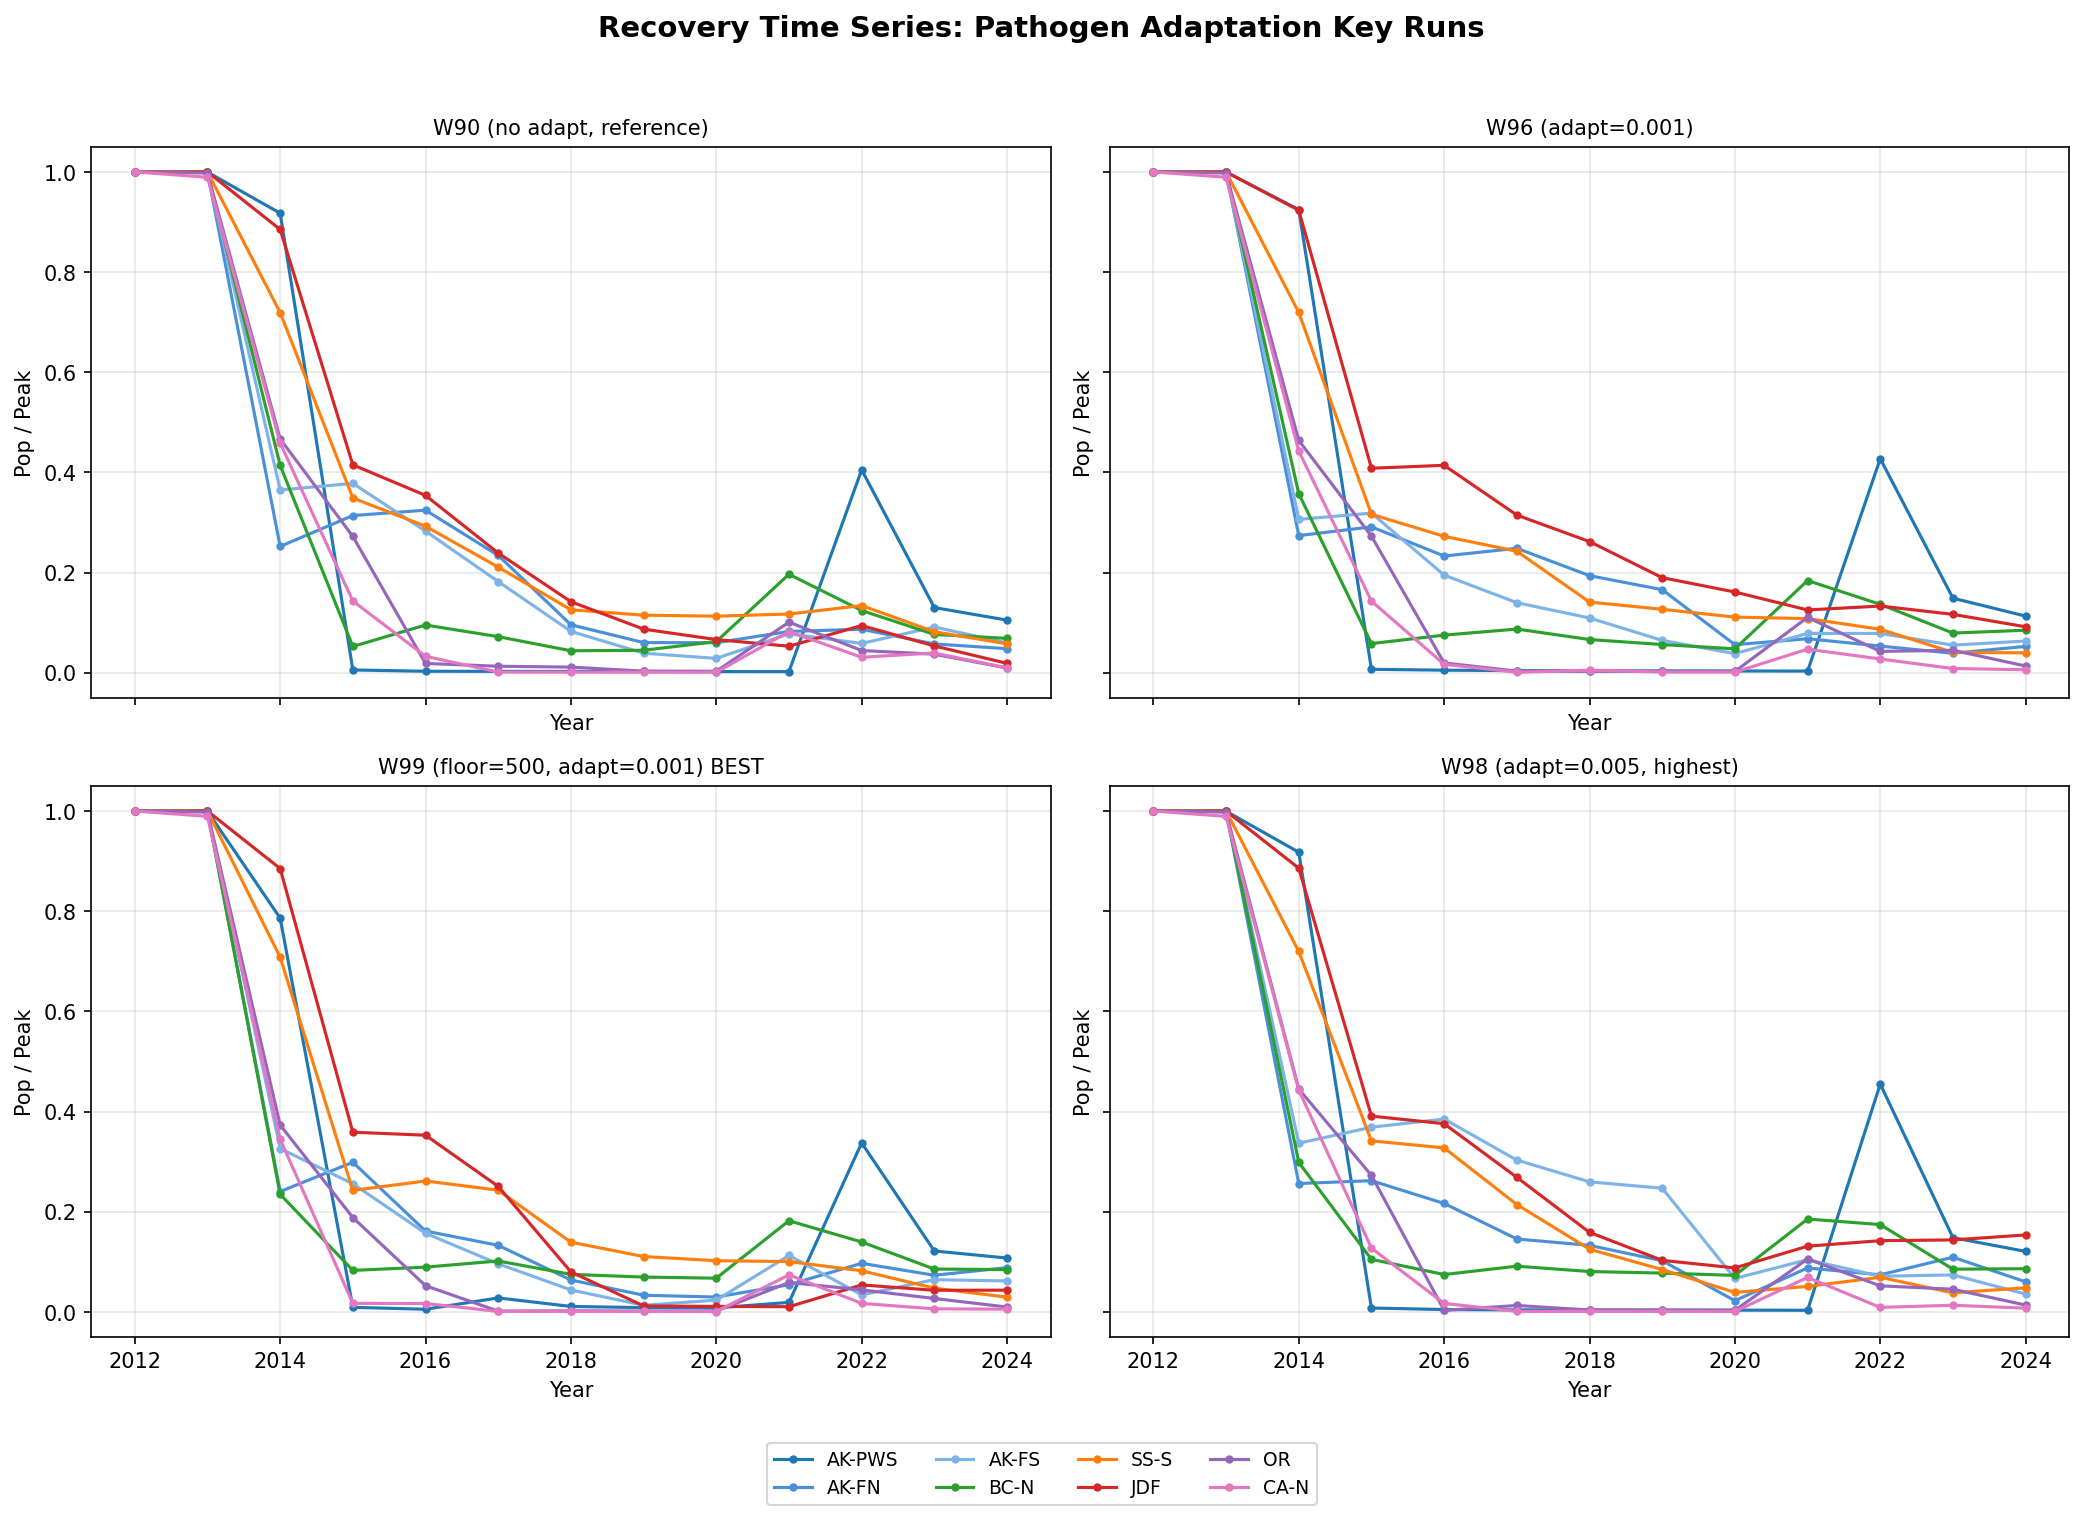
\includegraphics[width=\textwidth]{figures/fig1_key_runs.png}
\caption{Recovery trajectories for W90 (reference), W96 (adapt=0.001), W99 (best RMSE), W98 (highest adapt rate).}
\end{figure}

\subsection{All Runs Grid}
\begin{figure}[h]
\centering
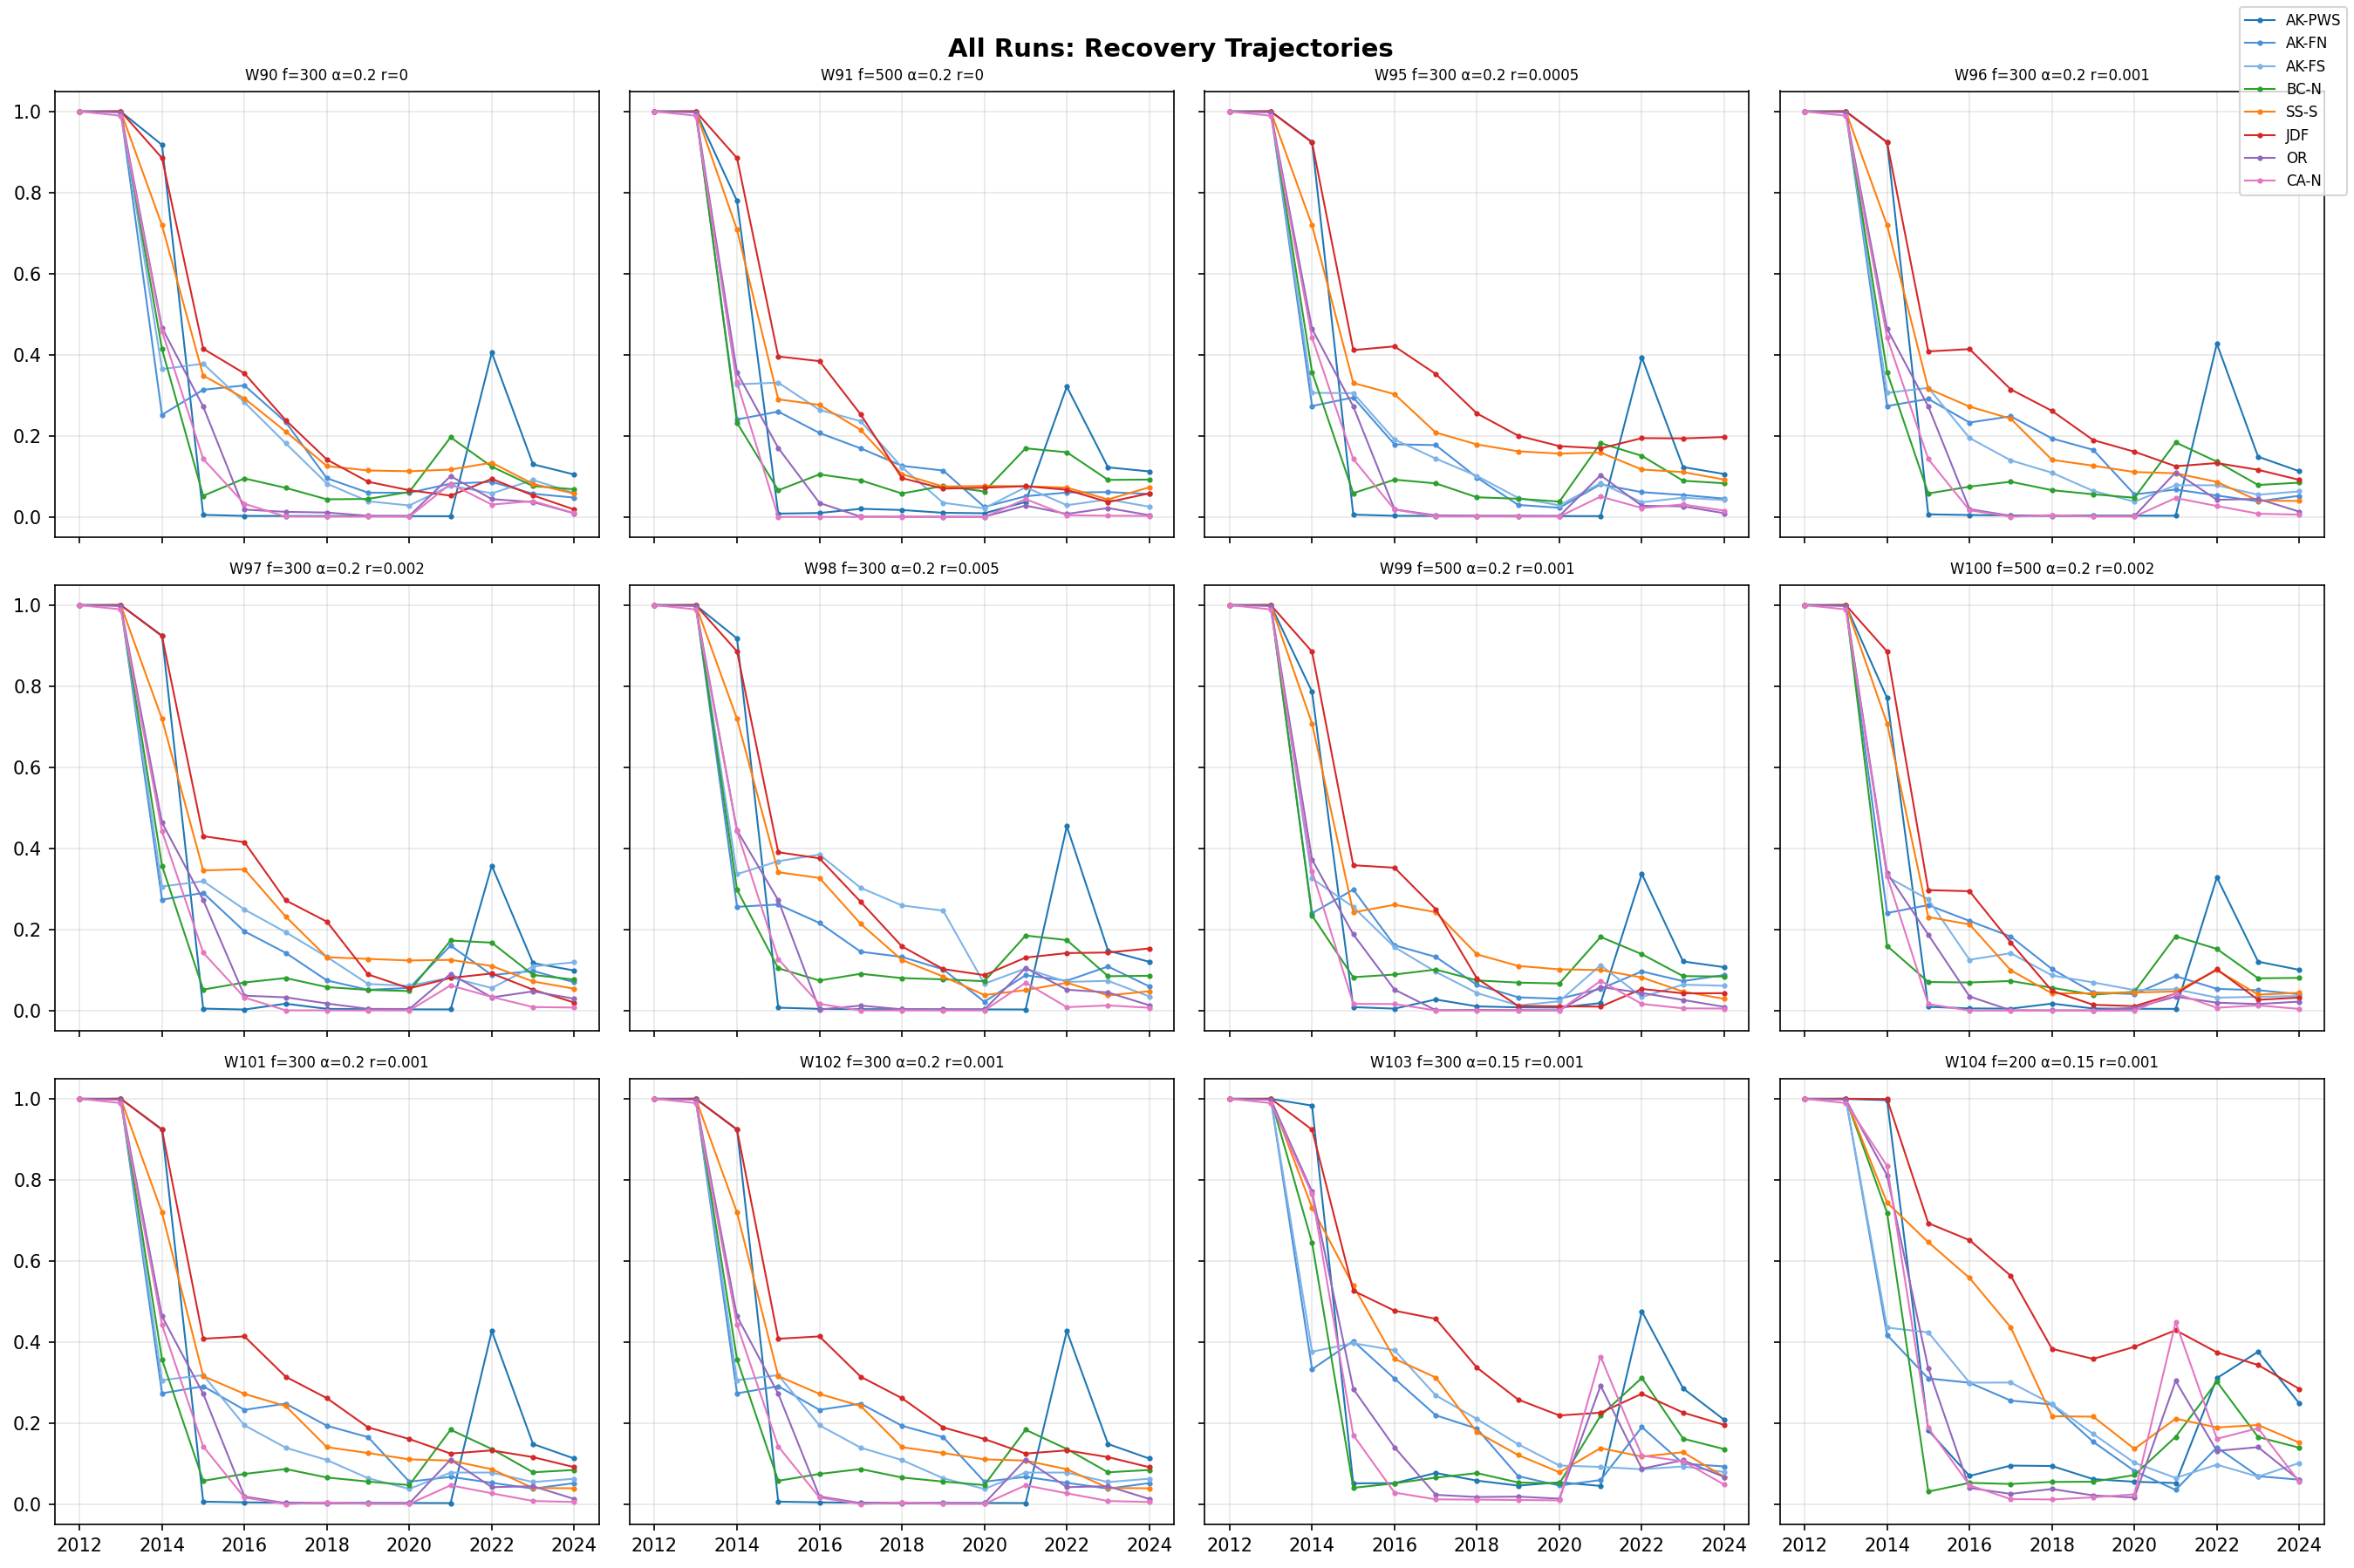
\includegraphics[width=\textwidth]{figures/fig2_all_runs.png}
\caption{All 12 runs (2 references + 10 adaptation runs).}
\end{figure}

\subsection{Adaptation Rate Effect}
\begin{figure}[h]
\centering
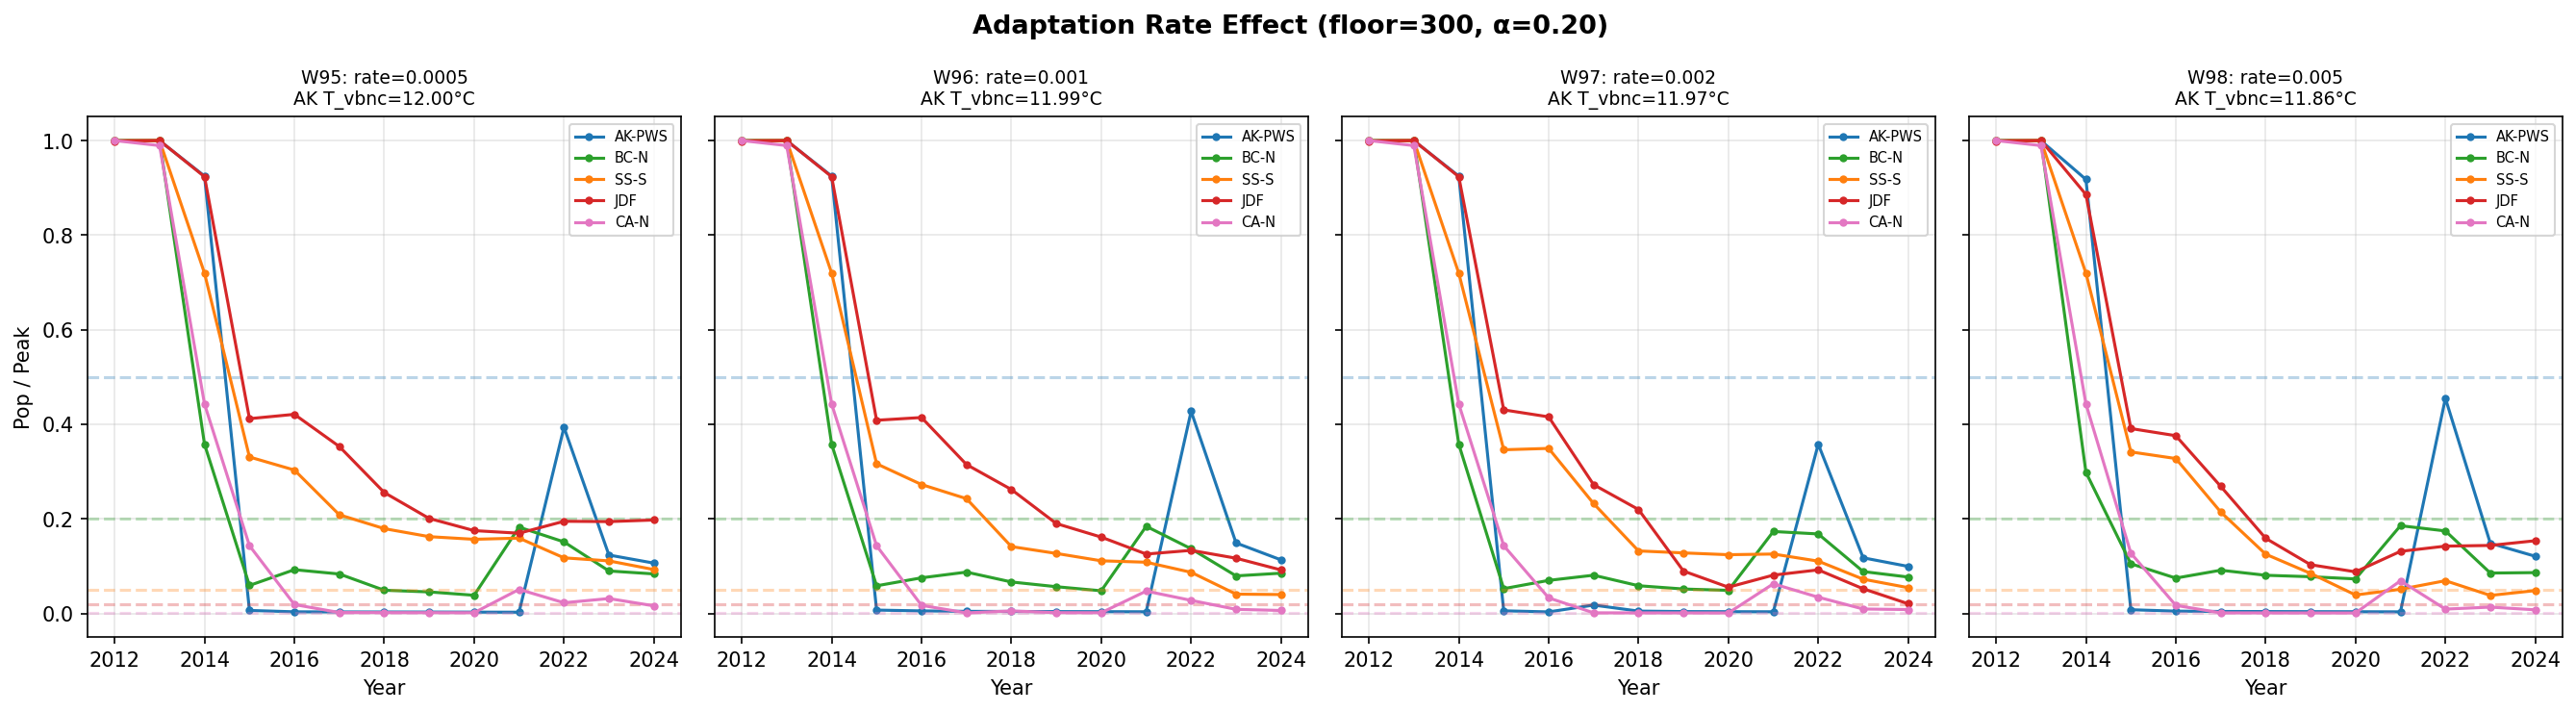
\includegraphics[width=\textwidth]{figures/fig3_adapt_rate.png}
\caption{Increasing adaptation rate (W95--W98). Note final $T_\mathrm{vbnc}$ values barely change.}
\end{figure}

\subsection{Recovery Comparison}
\begin{figure}[h]
\centering
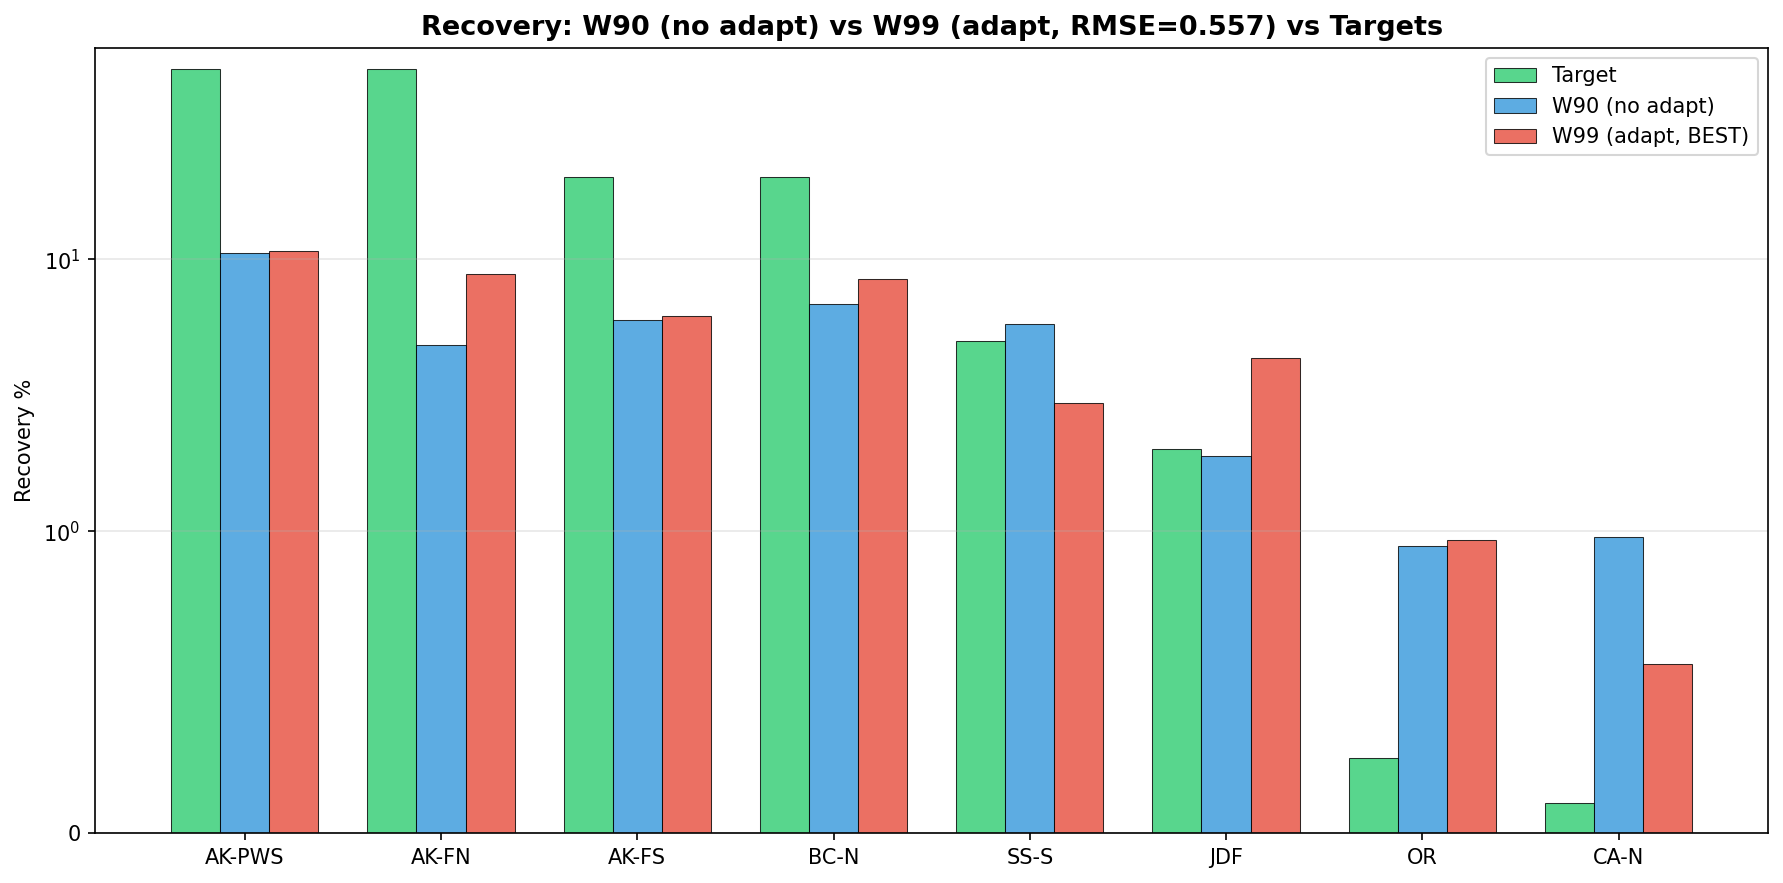
\includegraphics[width=\textwidth]{figures/fig4_bar_comparison.png}
\caption{W90 vs W99 vs targets. AK-PWS remains $\sim$5$\times$ below target.}
\end{figure}

\section{T\_vbnc Adaptation Analysis}

\begin{figure}[h]
\centering
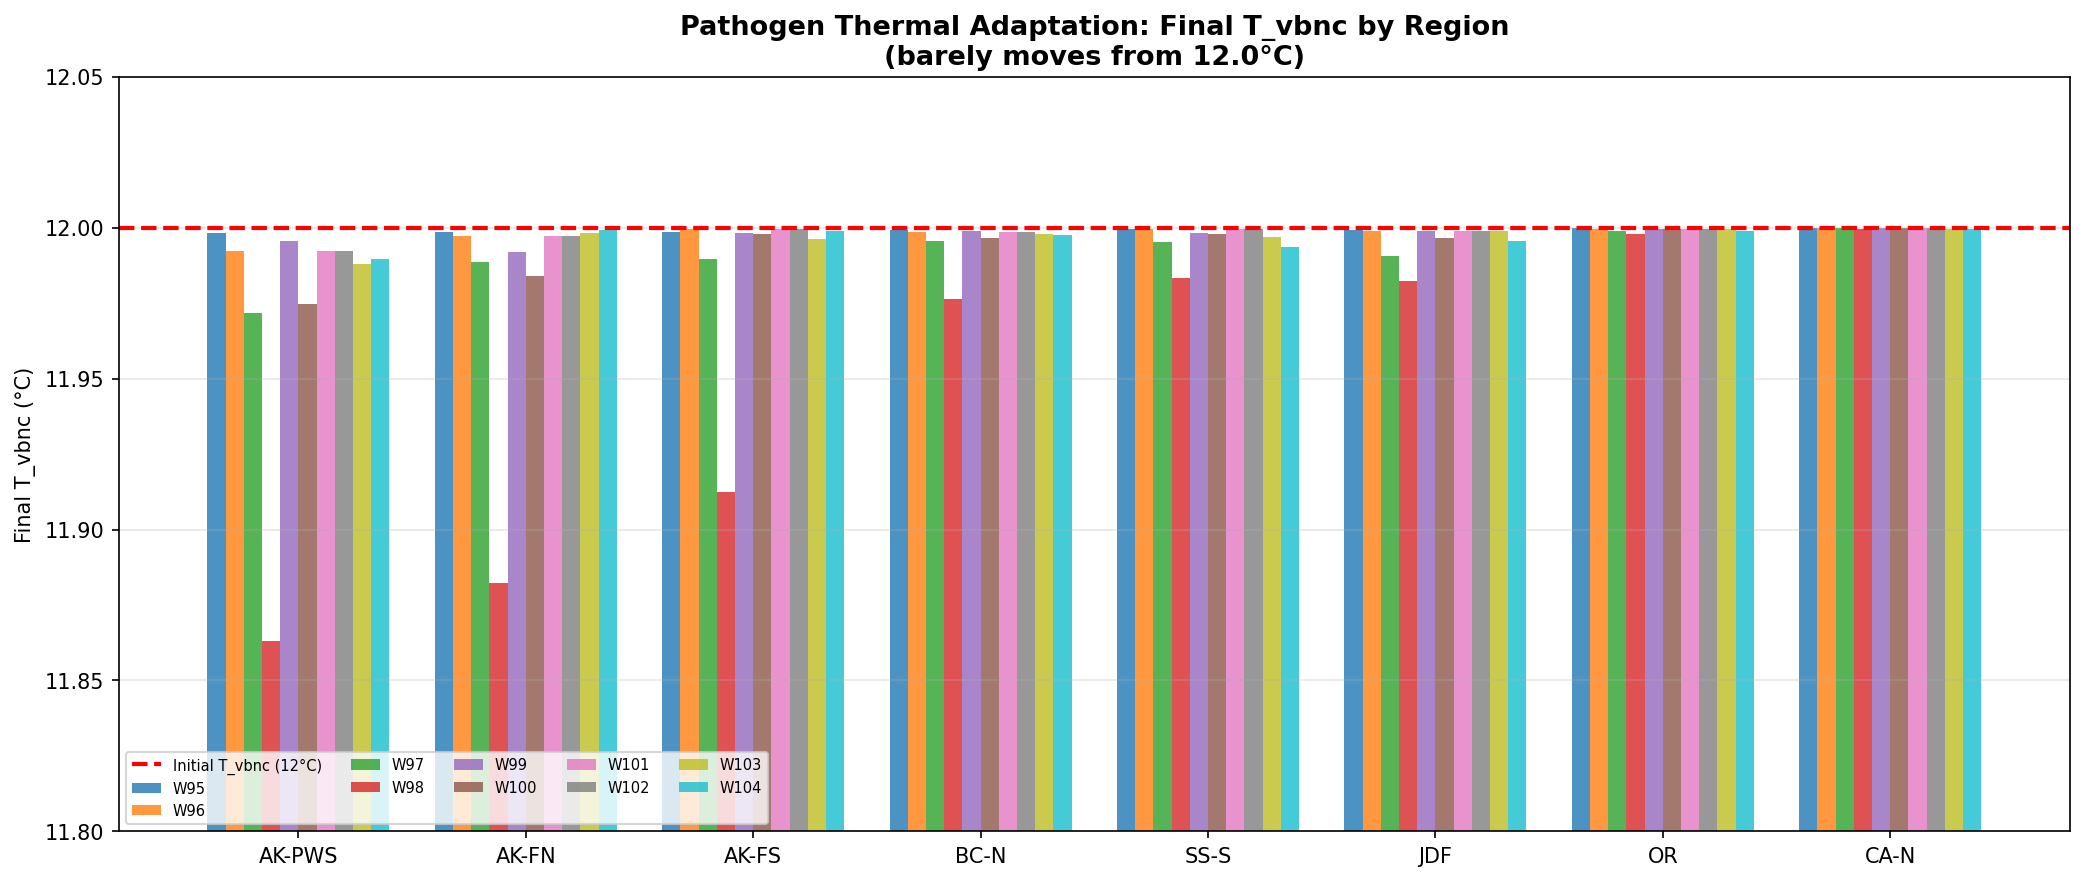
\includegraphics[width=\textwidth]{figures/fig5_tvbnc_adaptation.png}
\caption{\textbf{The key negative result}: Final $T_\mathrm{vbnc}$ per region across all adaptation runs. All values cluster within 0.15\textdegree C of the initial 12.0\textdegree C. The mechanism is inert at these rates.}
\end{figure}

\textbf{Why adaptation fails:} The daily adaptation is $\Delta T = r \times \mathrm{prevalence} \times (T_\mathrm{vbnc} - T)$. With prevalence $\sim$1--5\%, temp gap $\sim$2\textdegree C, and $r=0.001$: $\Delta T \approx 0.00002$\textdegree C/day $\approx$ 0.09\textdegree C over 13 years. Reversion (0.0005/day) further counteracts.

\subsection{T\_vbnc\_min Irrelevance}
\begin{figure}[h]
\centering
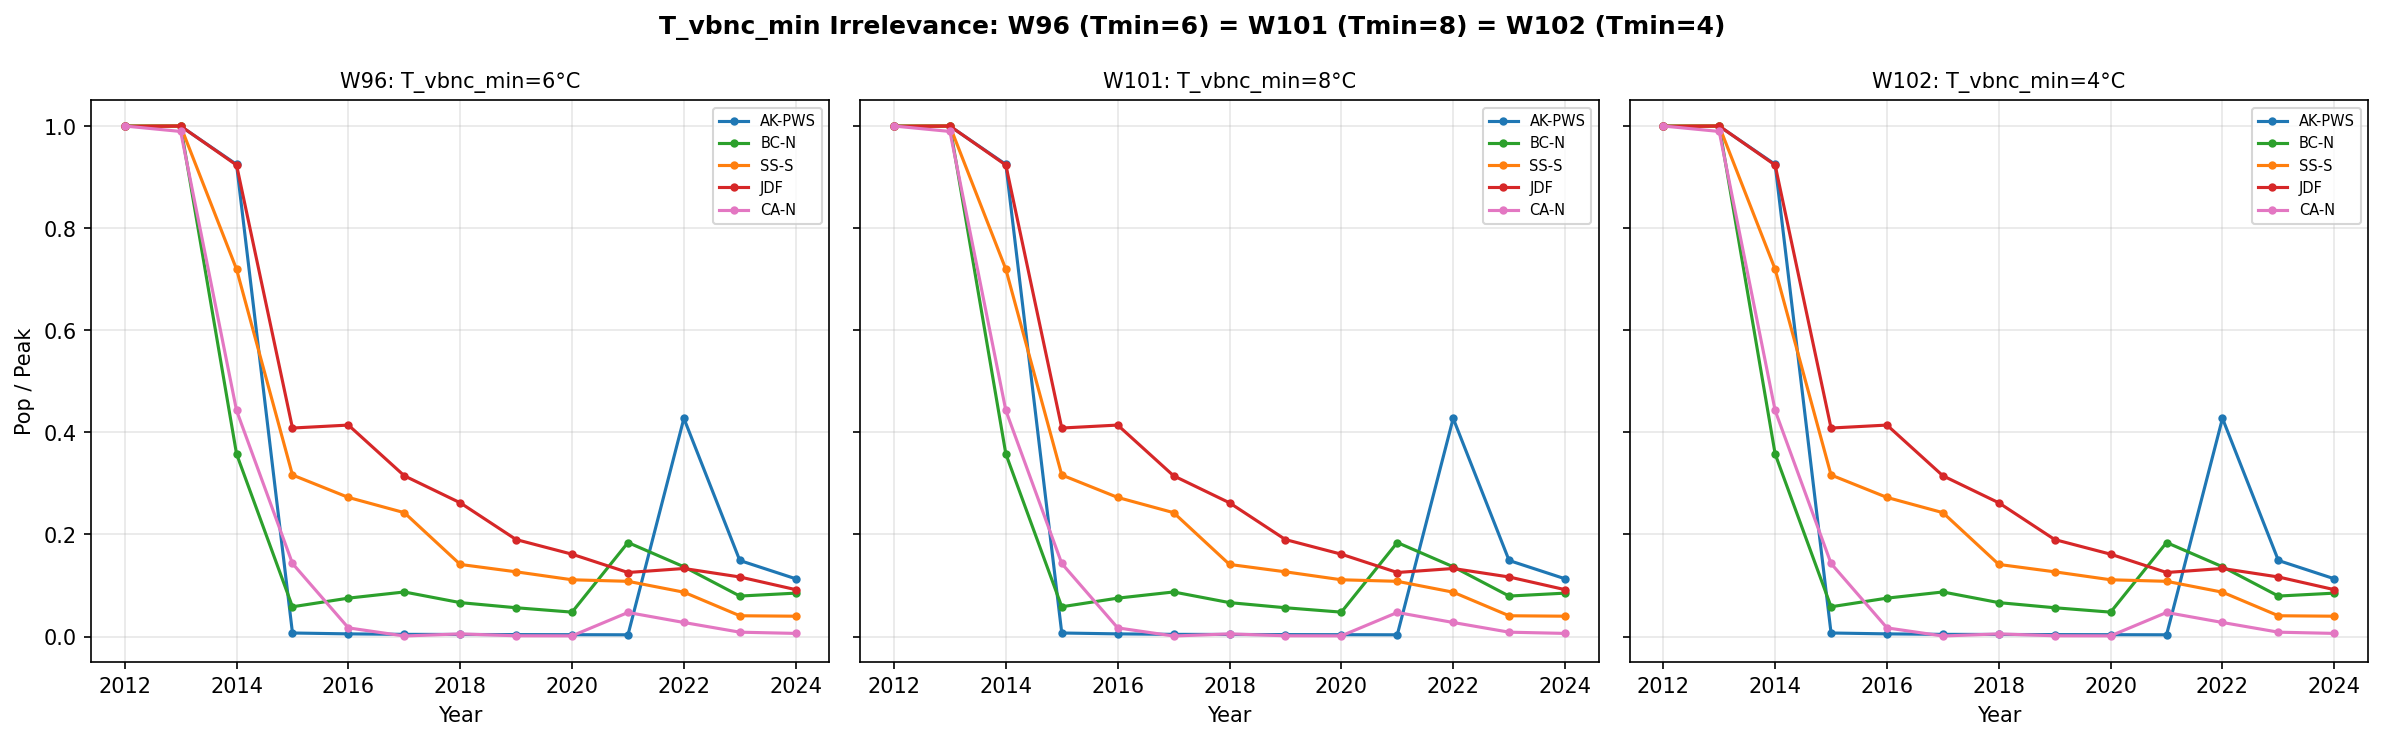
\includegraphics[width=\textwidth]{figures/fig7_tmin_irrelevance.png}
\caption{W96/W101/W102 produce \textit{identical} results despite $T_\mathrm{vbnc,min}$ = 6/8/4\textdegree C. The floor is never approached.}
\end{figure}

\section{RMSE Comparison}
\begin{figure}[h]
\centering
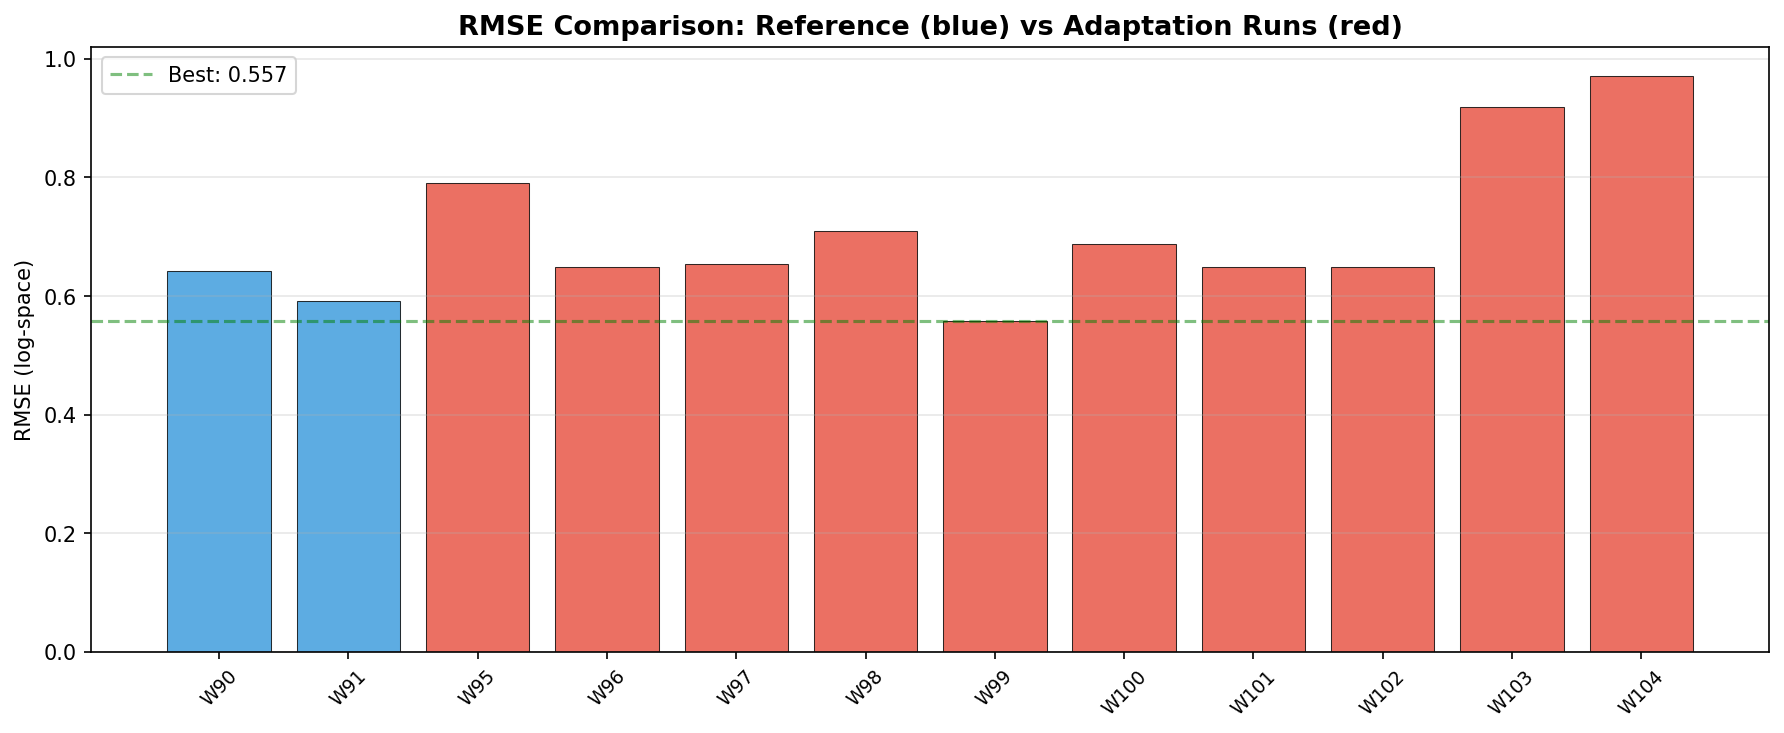
\includegraphics[width=\textwidth]{figures/fig6_rmse.png}
\caption{RMSE across all runs. W99 (0.557) is best, but improvement over W91 (0.591) is modest and not from adaptation.}
\end{figure}

\section{$\alpha_\mathrm{env}$ Effect}
\begin{figure}[h]
\centering
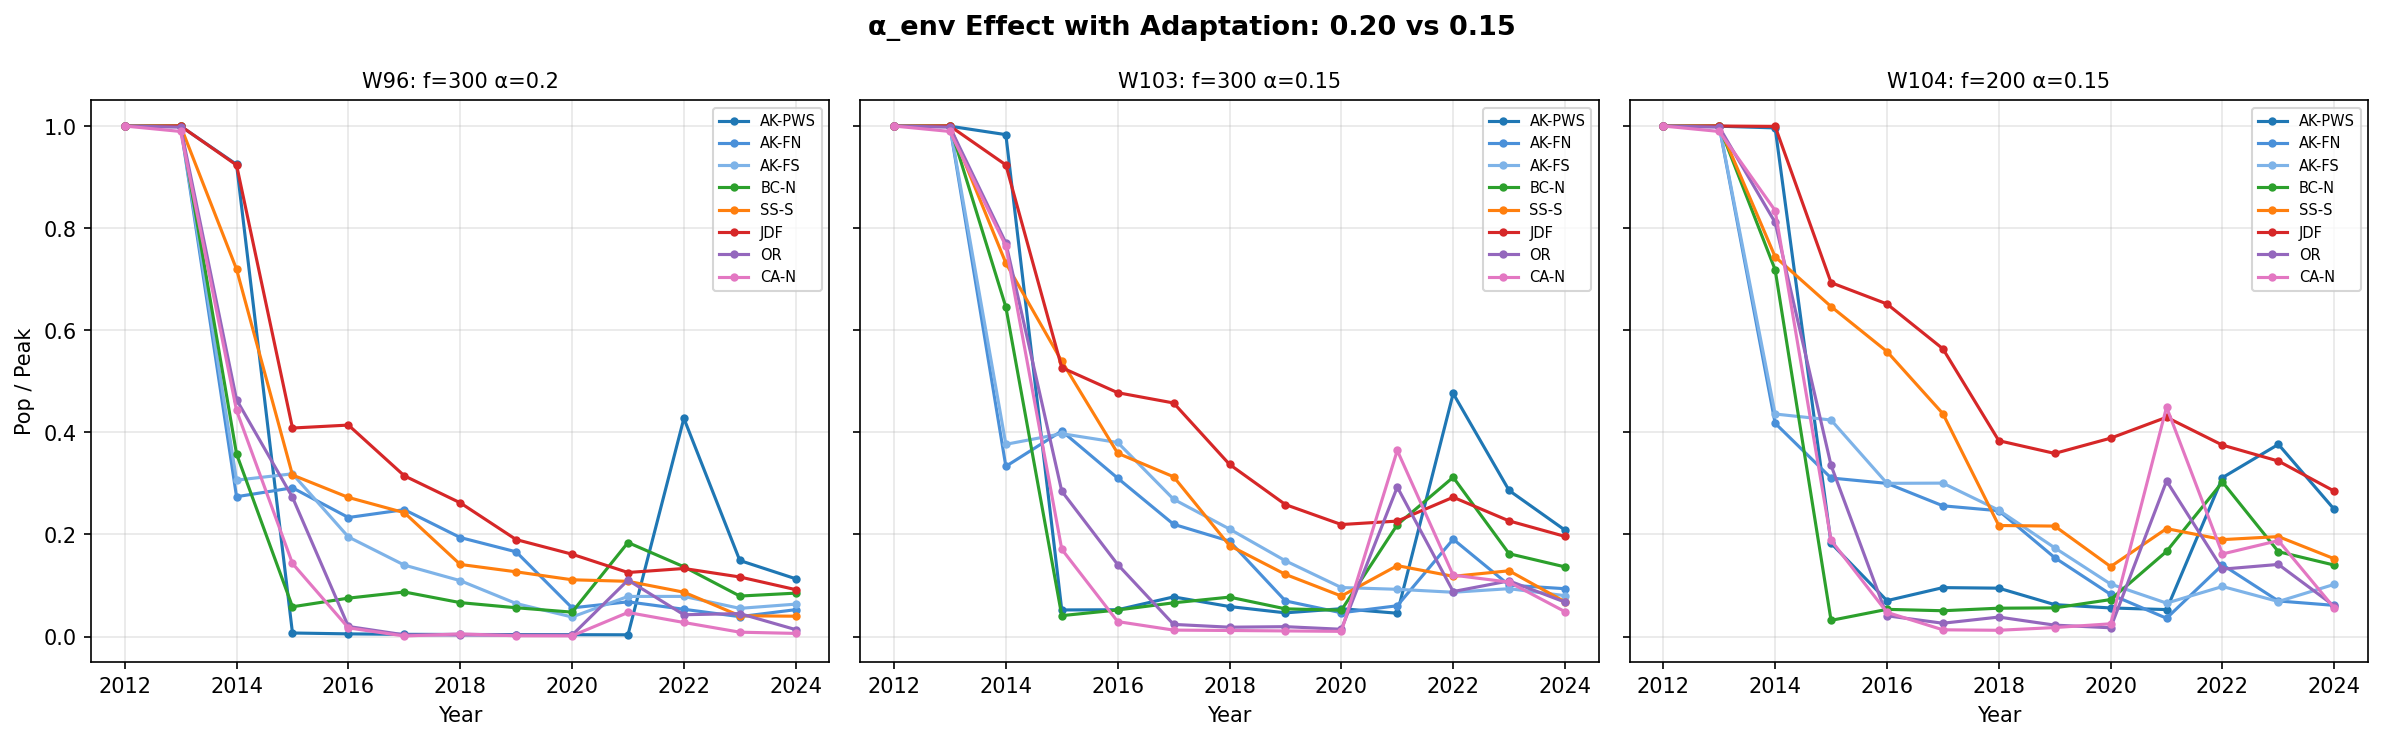
\includegraphics[width=\textwidth]{figures/fig8_alpha_effect.png}
\caption{$\alpha=0.15$ (W103/W104) vs $\alpha=0.20$ (W96). Lower $\alpha$ reduces gradient, inflates southern recovery.}
\end{figure}

\section{Key Findings}
\begin{enumerate}
\item \textbf{Pathogen adaptation is negligible} at biologically plausible rates over 13-year timescale
\item \textbf{$T_\mathrm{vbnc,min}$ is irrelevant} --- adaptation never approaches the biophysical floor
\item \textbf{W99 achieves RMSE=0.557} (best ever) due to floor=500 + $\alpha$=0.20, not adaptation
\item \textbf{Alaska recovery remains the core problem}: 10--12\% across all runs vs 50\% target
\item \textbf{$\alpha_\mathrm{env}$ dominates}: $\alpha$=0.20 produces strong gradient; $\alpha$=0.15 destroys it
\end{enumerate}

\section{Implications}
The mechanism as designed (prevalence-scaled daily increments) is too slow. Two paths forward:
\begin{itemize}
\item \textbf{Redesign}: Model strain \textit{replacement} rather than gradual adaptation --- binary or threshold-based rather than continuous
\item \textbf{Refocus}: Accept that the north-south gradient comes from dynamic $P_\mathrm{env}$ (floor + $\alpha$) and focus on lifting Alaska recovery through other mechanisms (recruitment, $K_{1/2}$, settler survival)
\end{itemize}

\end{document}
